\subsection{Candidate Ranking}
\label{sec:ranking}


It is possible that multiple SQL queries satisfying
the given input-output examples will be returned.
To help end-users select their expected queries,
\ourtool ranks more likely queries higher in the output.
%This may adversely impact end-users who want to
%perform simple query tasks but now need
%to select the query of their intent.
%To alleviate this problem, 
Specifically, \ourtool employs
the Occam's razor principle, which states that the
simplest explanation is usually the correct one.
A simpler query is less likely to overfit the given examples
than a complex query, even when both of them
can transform the example input to the example output.


%We define a comparison scheme between different
%SQL queries by defining a partial order between them. Some of
%these choices are subjective, but have been observed to work well.
A SQL query is simpler than another one if it uses
fewer query conditions (including conditions in the \CodeIn{Having}
and \CodeIn{from} clauses) or the expressions (including
aggregates) in each query condition or clause are pairwise simpler.
For example, expression \CodeIn{Count(student\_id)} is simpler than
\CodeIn{Count(Distinct student\_id)}.
Simpler query conditions and expressions often suggest the extraction logics
are more common and general.

In our implementation, \ourtool computes a cost for each
query, and prefers queries with lower costs. The cost
for a SQL query is computing approximately by summarizing
the number of conditions, aggregates,
and other expressions
appearing in the \CodeIn{GROUP BY} and \CodeIn{ORDER BY} clauses.
This heuristic has been observed
to work well.
Figure~\ref{fig:rank} shows an example.


\begin{figure}[t]
\centering
 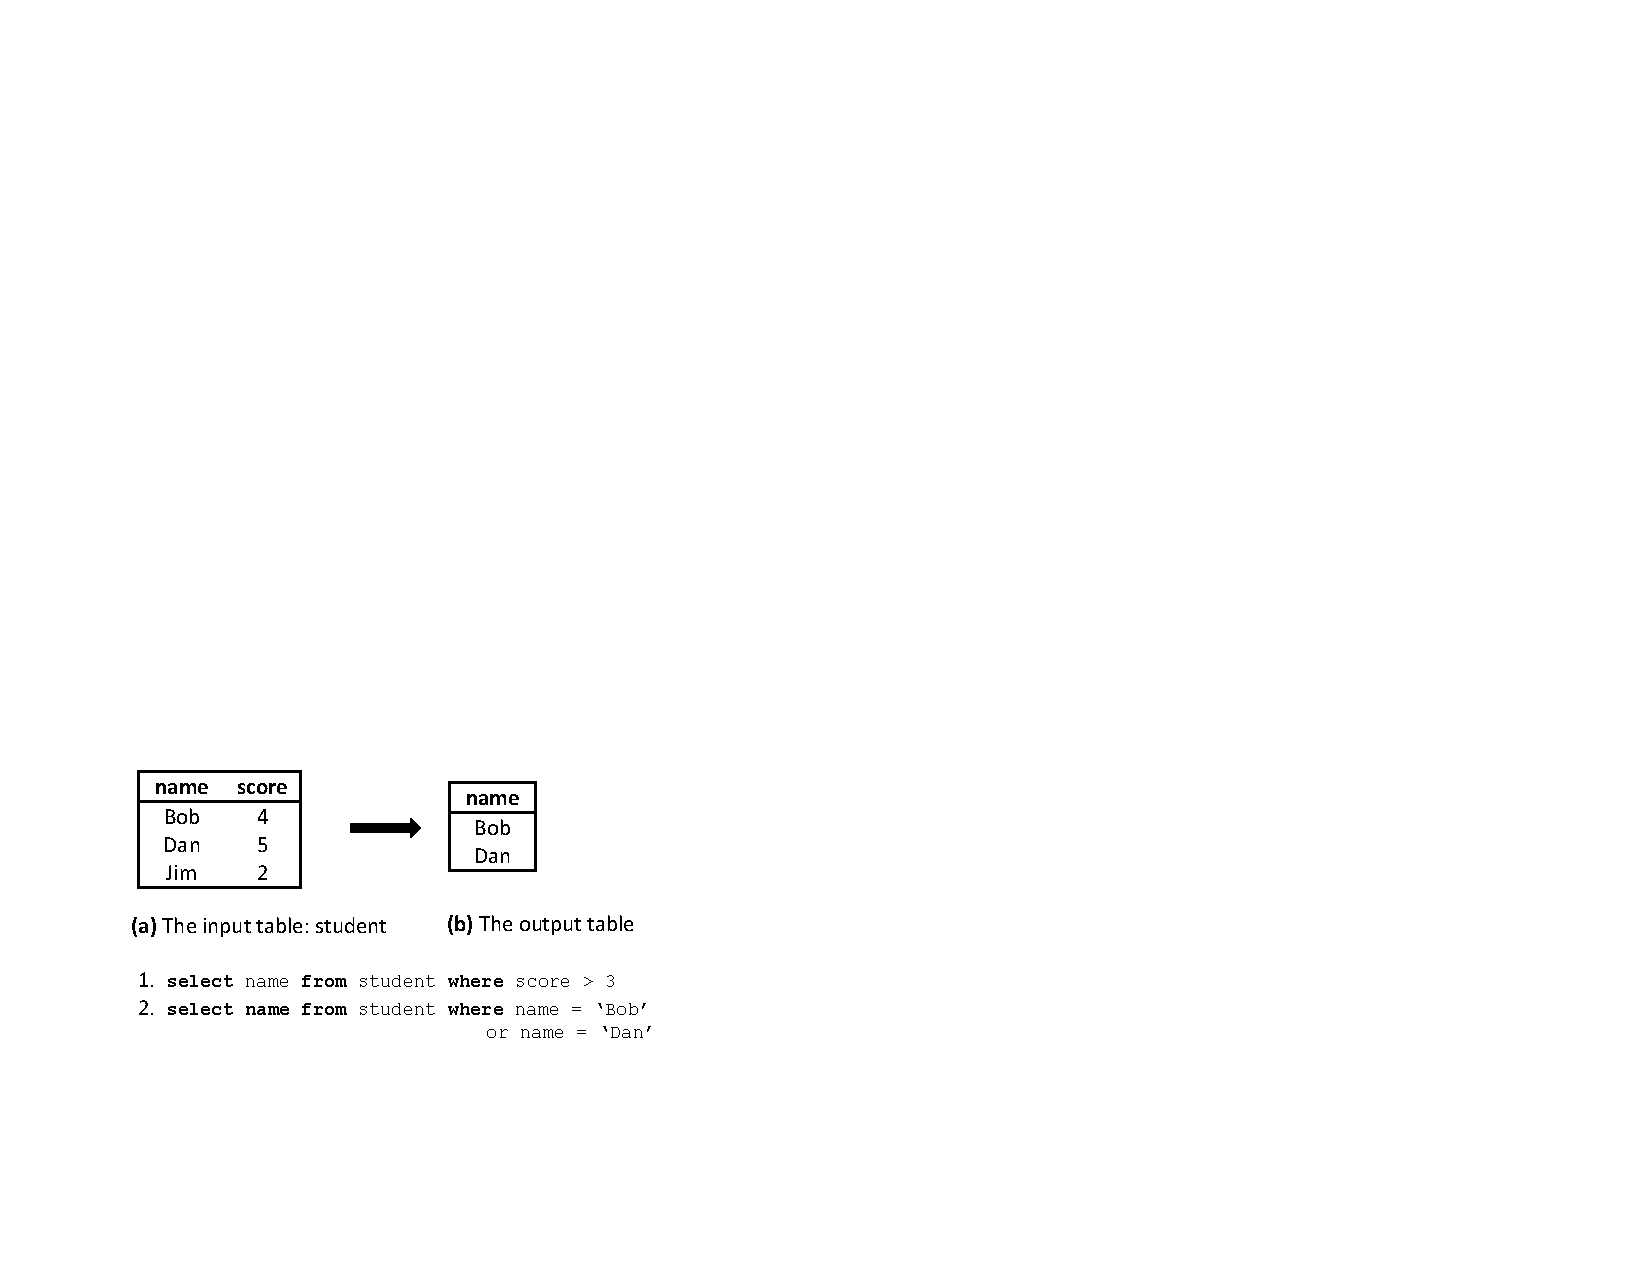
\includegraphics[scale=0.80]{rankexample}
 \vspace{-3mm}
\Caption{{\label{fig:rank} Illustration of \ourtool's
query candidate ranking heuristic. \ourtool produces two
queries for the given input-output examples. Based on
the heuristic in Section~\ref{sec:ranking}, the first query
differs from the second query by using simpler conditions,
and thus is ranked higher.
}}
\end{figure}

